% Chapter 2

\chapter{Methodology} % Main chapter title

\label{Chapter2} % For referencing the chapter elsewhere, use \ref{Chapter2} 

%----------------------------------------------------------------------------------------

\section{Supervised learning architecture for speech enhancement}
Supervised learning is the machine learning task of learning a function that maps an input to an output based on example input-output pairs \cite{wiki:sl}. In supervised learning, each example is a pair consisting of an input object and a desired output value (also called the supervisory signal). A supervised learning algorithm analyzes the training data and produces an inferred function, which can be used for mapping new examples.\par
The idea of using supervised learning for speech-enhancement involves using the training data consisting of audio features as input object and the desired t-f mask as an output value during the training phase (See figure: \ref{fig:training_layout}). This would enable a deep learning model to learn a function to model the training data. The trained deep learning model can then be used on a testing dataset that would only involve audio features as input to the trained deep learning model. Post training phase, the deep learning model would then predict the t-f mask for the input audio features (See figure: \ref{fig:testing_layout}).\par
\begin{figure}
\centering
\begin{subfigure}{.5\textwidth}
  \centering
  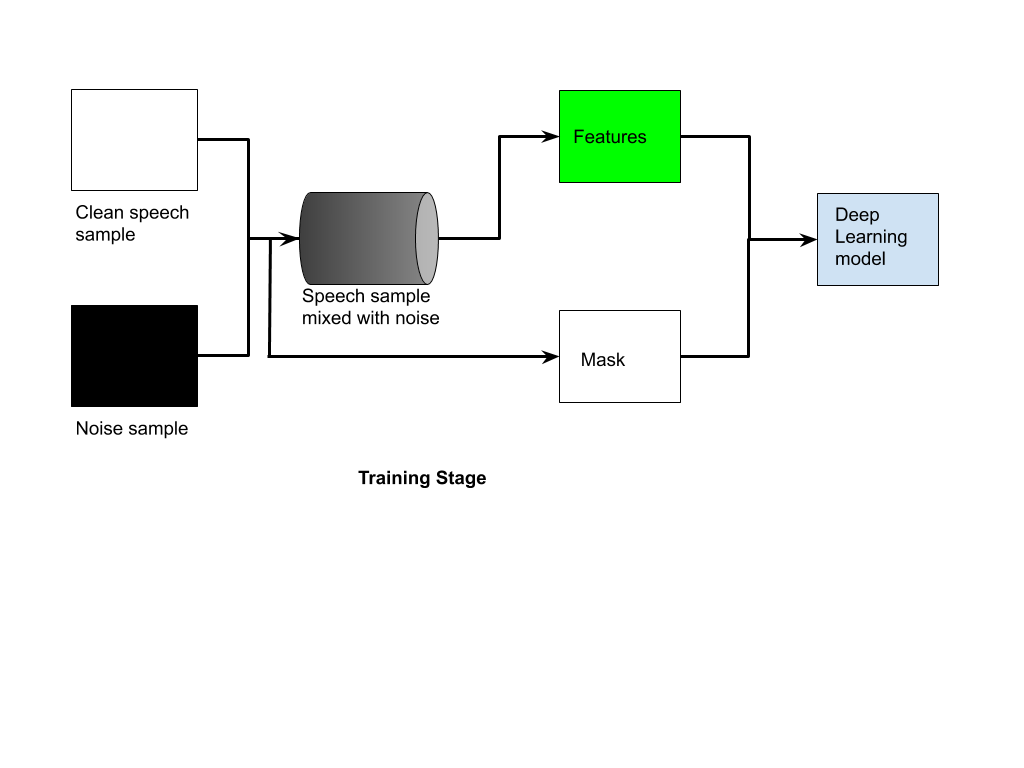
\includegraphics[width=1.25\linewidth]{training_layout}
  \caption{Training Stage Layout}
  \label{fig:training_layout}
\end{subfigure}%
\begin{subfigure}{.5\textwidth}
  \centering
  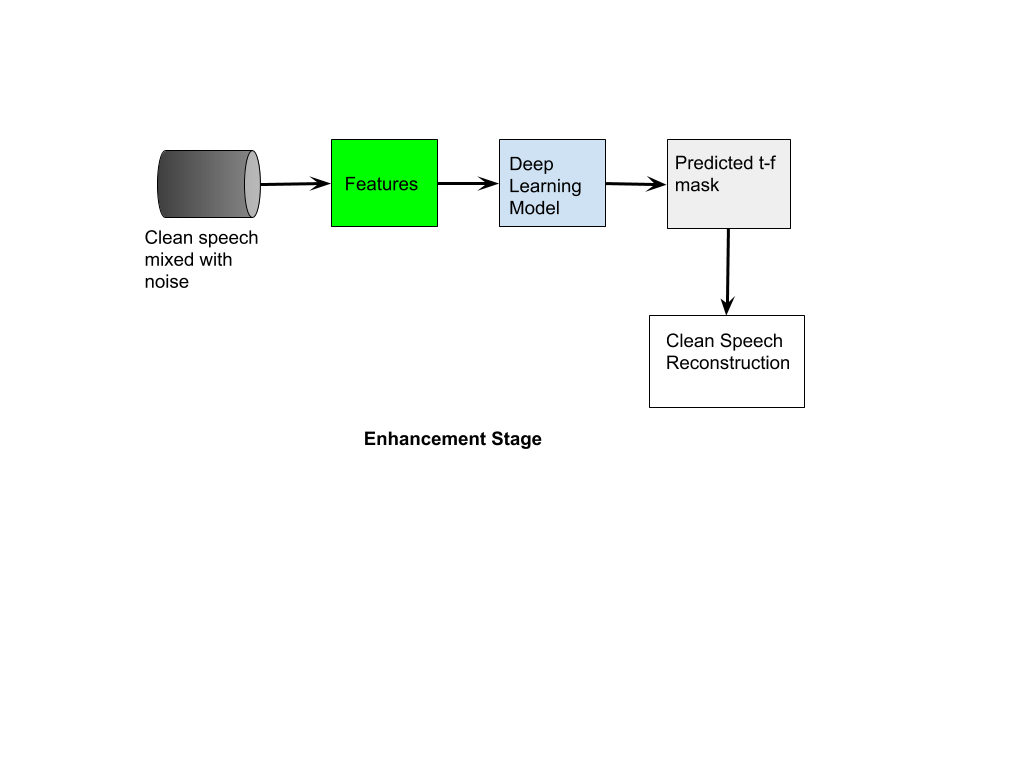
\includegraphics[width=1.25\linewidth]{testing_layout}
  \caption{Testing Stage Layout}
  \label{fig:testing_layout}
\end{subfigure}
\caption{Deep Learning based speech enhancement layouts}
\label{fig:layouts}
\end{figure}
%----------------------------------------------------------------------------------------
\section{Dataset}
Dataset forms the most important part of any supervised learning problem. For the experiments in this project, only the speech portion, which consists of read speech (TIMIT recordings), and the set of noises(MUSAN recordings), which ranges from beeps emitted from technical equipment, to ambient sounds such as rain, road , factory noise, etc) were considered. All of the files are available in \enquote{.wav} format, are single channel, and are 16 bit sample PCM encoded. All recordings are downsampled to 8kHz sampling rate to speed up the training phase.

\begin{itemize}
\item \textbf{Clean Speech Dataset}:\\
\textbf{\href{http://www.ldc.upenn.edu/Catalog/CatalogEntry.jsp?catalogId=LDC93S1}{TIMIT}}: This corpus \cite{ref:timit} consists of a total of 1700 sentences spoken by roughly 630 speakers of eight major dialects of American English. TIMIT corpus includes time-aligned orthographic, phonetic and word transcriptions as well as a 16-bit, 16kHz speech waveform file for each utterance. To speed up the training in our case however, these samples were downsampled to 8kHz. Corpus design was a joint effort among the Massachusetts Institute of Technology (MIT), SRI International (SRI) and Texas Instruments, Inc. (TI). The speech was recorded at TI, transcribed at MIT and verified by the National Institute of Standards and Technology (NIST).
\item \textbf{Noise Dataset}:\\
\textbf{\href{https://www.openslr.org/17/}{MUSAN}}: This is a corpus of music, speech, and noise recordings \cite{ref:musan2015}. This dataset consists of music, speech recordings in twelve different languages, and a large set of naturally occuring and technical noises. Its primary intention is that of being a training corpus for voice activity detection. We considered the noise sub set of this corpus which amounts to around 6 hours of the duration.
\end{itemize}

\subsection{Generation of Noisy Mixture}
During training phase, the clean speech sample was mixed with a randomly chosen noise sample after making both samples of same duration and at the same amplitude level, i.e. both clean speech and noise samples were first normalised to have same amplitude and then added together. The mixing procedure has been depicted as a flow chart in the figure \ref{fig:gen_mix}.

\begin{figure}[!htbp]
\centering
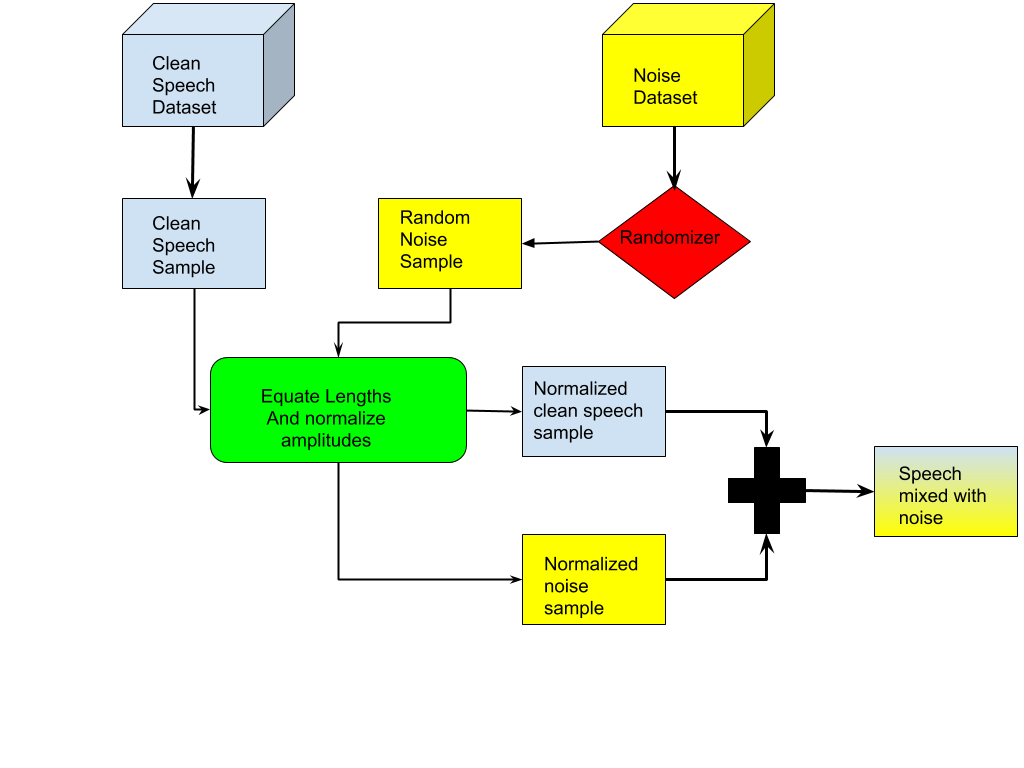
\includegraphics[width=1.15\linewidth]{gen_mix}
\caption{Generation of Noisy speech samples}
\label{fig:gen_mix}
\end{figure}

%---------------------------------------------------------------------------
\section{Features}
In machine learning and pattern recognition, a feature is an individual measurable property or characteristic of a phenomenon being observed \cite{wiki:feat}. Choosing informative, discriminating and independent features is a crucial step for effective algorithms in pattern recognition, classification and regression. \par Features as input and learning machines play complementary roles in supervised learning. When features are discriminative,they place less demand on the learning machine in order to perform a task successfully. On the other hand, a powerful learning machine places less demand on features.\par We conducted a study to examine different acoustic features for supervised speech enhancement:

\subsection{\textbf{Spectrogram}}
A spectrogram is a visual representation of the spectrum of frequencies of a signal as it varies with time. Spectrogram for an audio is constructed by combining the STFT at subband levels. Audio samples at 8 K\si{\hertz} are divided into frames of 30 m\si{\second}. Hence, each frame has 240 samples for which STFT is calculated. An overlap of 60 samples in adjacent frames is also used to reduce the effect of windowing. Combining STFT for all subband frames gives a spectrogram which can then be used as the training data and for generating spectrogram masks (See figure: \ref{fig:spect}).
\begin{figure}
\centering
\begin{subfigure}{.4\textwidth}
  \centering
  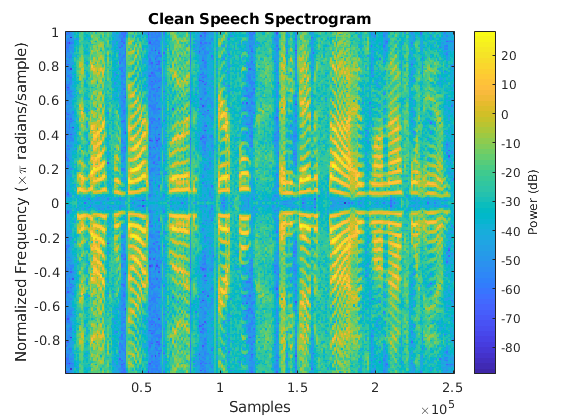
\includegraphics[width=1.1\linewidth]{clean_spect}
  \caption{Clean Speech Spectrogram}
  \label{fig:clean_spect}
\end{subfigure}%
\begin{subfigure}{.4\textwidth}
  \centering
  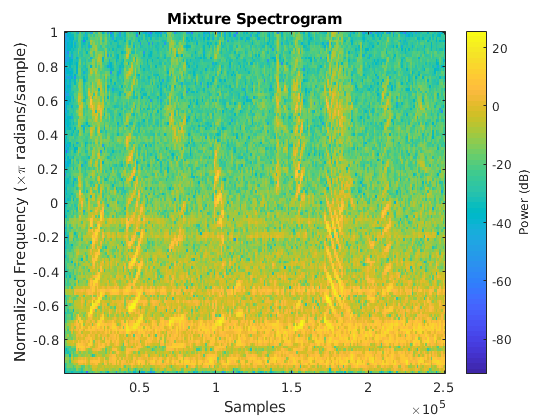
\includegraphics[width=1.1\linewidth]{mix_spect}
  \caption{Noisy mixture spectrogram}
  \label{fig:mix_spect}
\end{subfigure}
\begin{subfigure}{.4\textwidth}
  \centering
  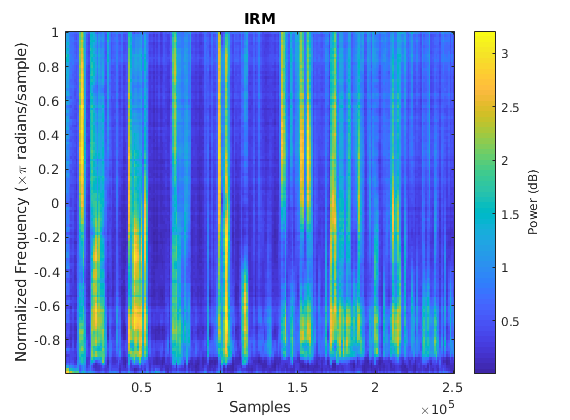
\includegraphics[width=1.1\linewidth]{IRM_spect}
  \caption{IRM - by learning model}
  \label{fig:irm_spect}
\end{subfigure}
\begin{subfigure}{.4\textwidth}
  \centering
  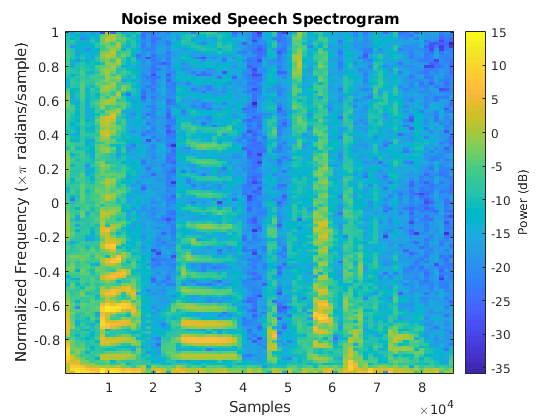
\includegraphics[width=1.1\linewidth]{estimated_spect}
  \caption{Estimated speech spectrogram}
  \label{fig:est_spect}
\end{subfigure}
\caption{Different stages of spectrogram during speech enhancement}
\label{fig:spect}
\end{figure}

\subsection{\textbf{GFCC}}
GFCC (Gammatone Frequency Cepstral Coefficients) are the gammatone-domain cepstrum based audio feaures. Being a cepstral property, it is a spectral representation of the spectrum of a time domain audio signal which has been filtered using a gammatone filterbank. These features are calculated at subband levels for frames of length 30ms. For an audio sampled at 8K\si{\hertz} rate, this imply 240 samples per frame. To reduce the effect of windowing, an overlap of 60 samples in adjacent frames is considered. This method to calculate GFCC, the rate of change of GFCC called GFCC delta and rate of change of GFCC delta, called GFCC double delta is described in \ref{fig:gfcc_extraction}. In all 13 gammatone frequency cepstral coefficients were considered (See figure: \ref{fig:gfcc_plot} \cite{mathworks:gtcc}).  

\begin{figure}
\centering
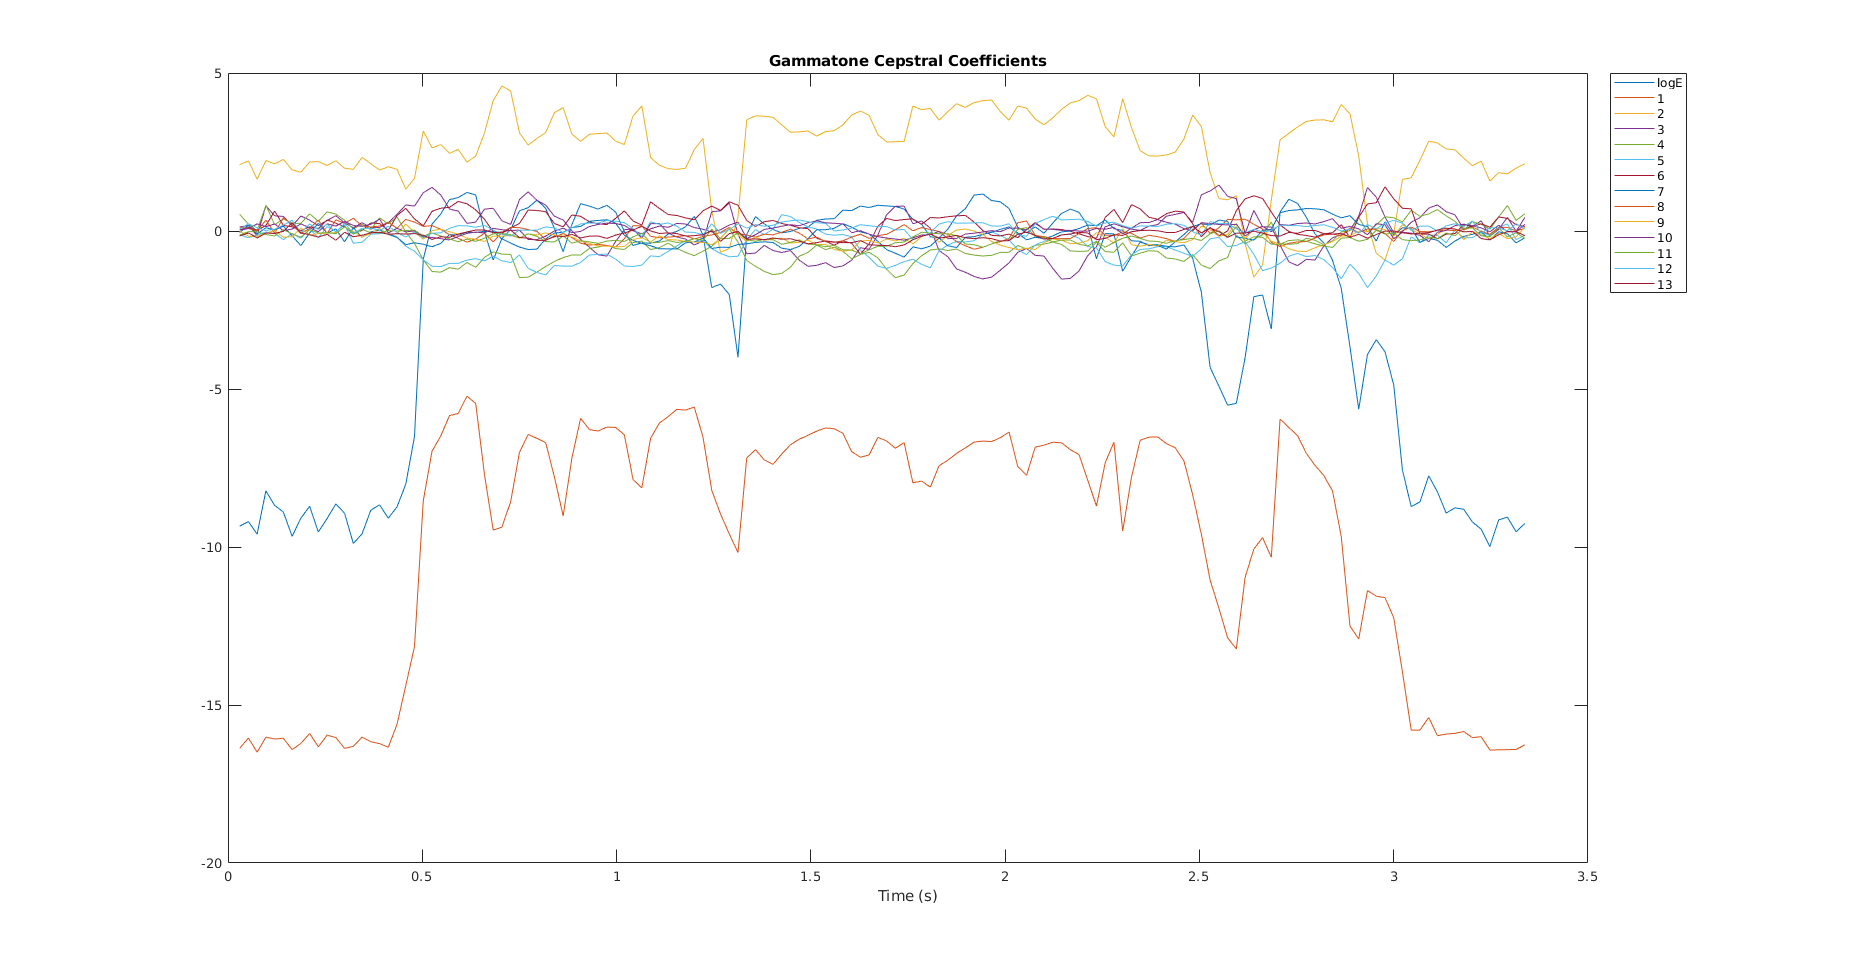
\includegraphics[width=1.15\linewidth]{gfcc_plot}
\caption{Typical GFCC plot with log energy and 13 coefficients}
\label{fig:gfcc_plot}
\end{figure}

\begin{figure}
\centering
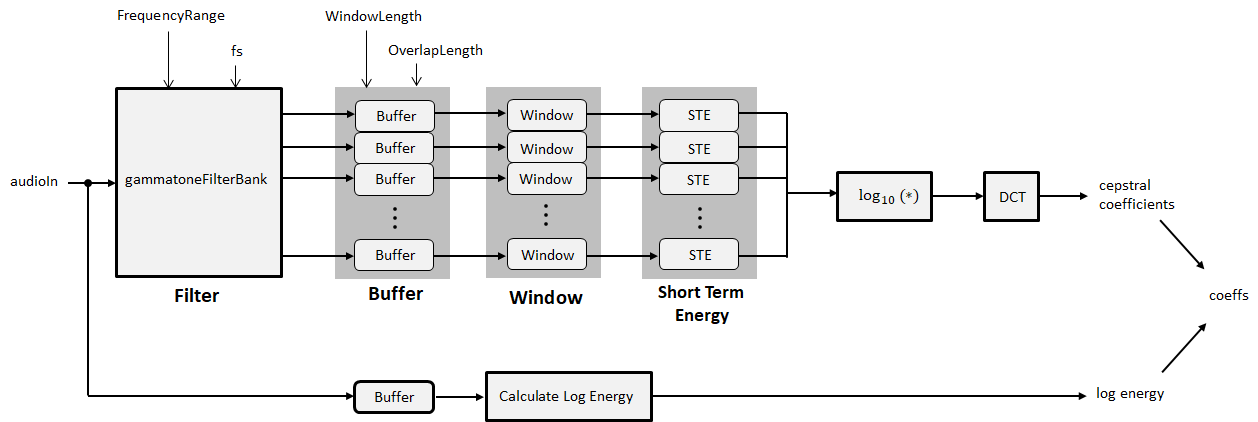
\includegraphics[width=1.2\linewidth]{gtcc_algorithm}
\caption{GFCC Extraction}
\label{fig:gfcc_extraction}
\end{figure}

\begin{figure}
\centering
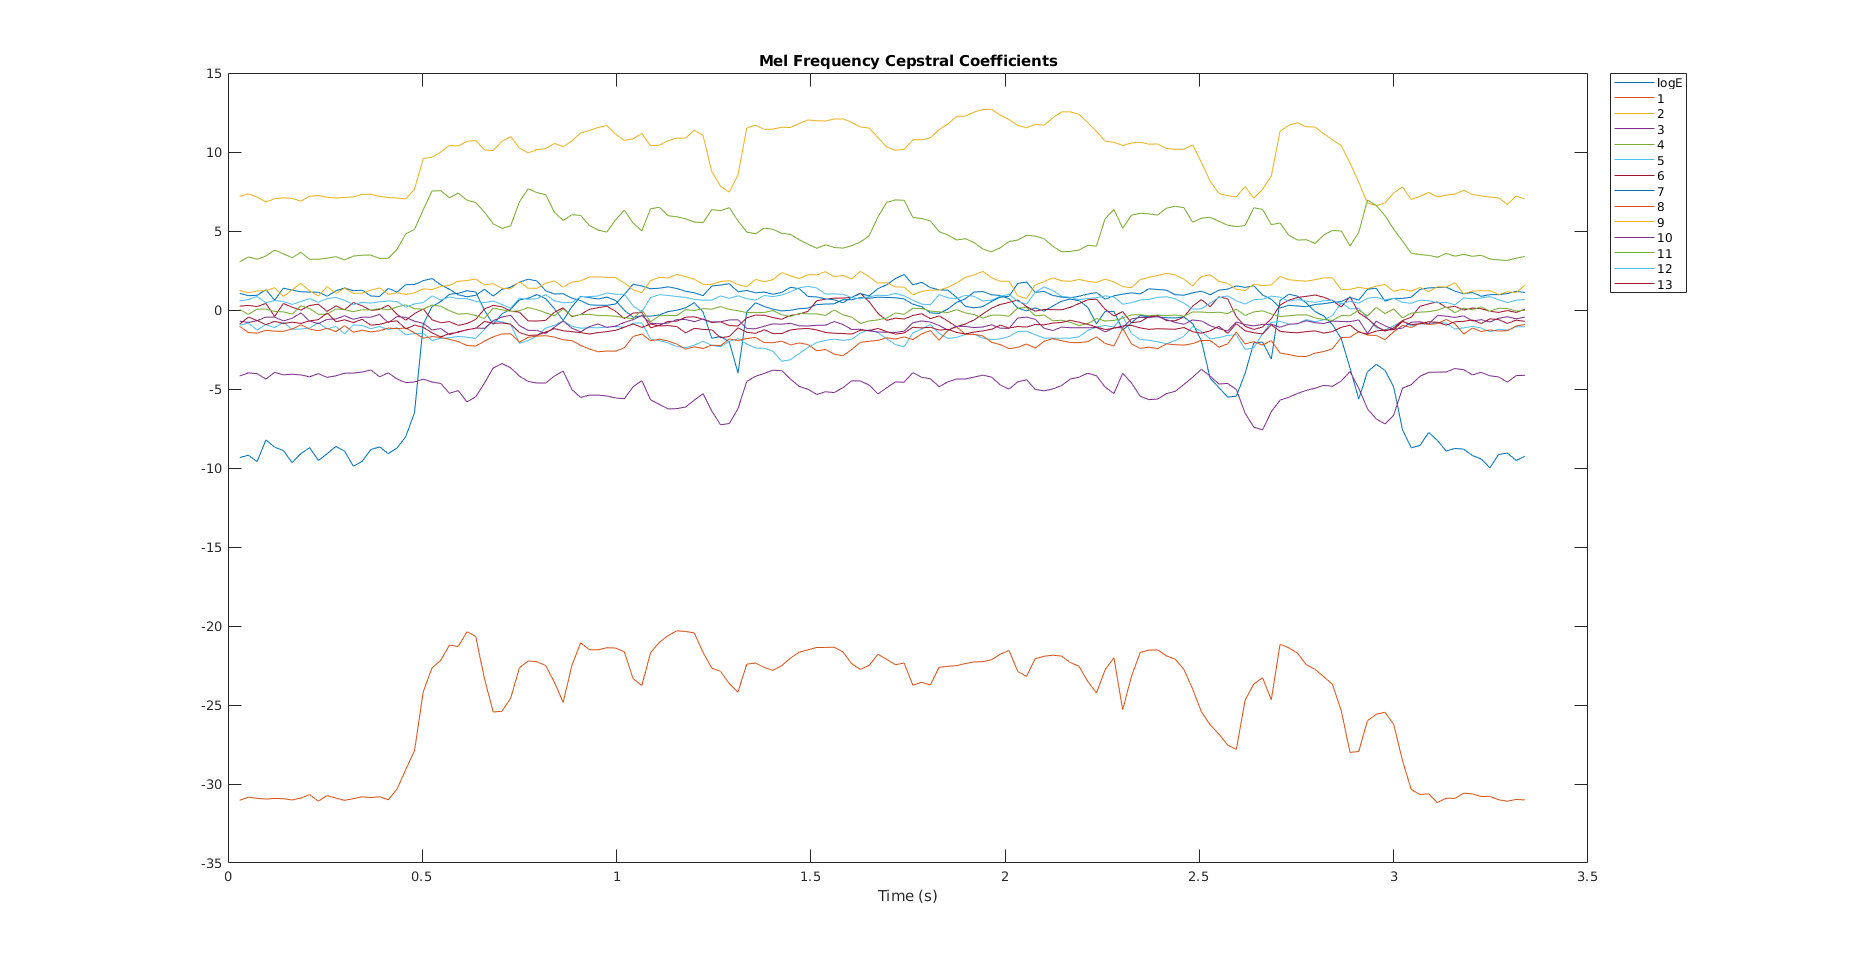
\includegraphics[width=1.25\linewidth]{mfcc_plot}
\caption{Typical MFCC plot with log enery and 13 coefficients}
\label{fig:mfcc_plot}
\end{figure}

\subsection{\textbf{MFCC}}
MFCC (Mel-Frequency Cepstral Coefficients) are the Mel-domain cepstrum based audio features. It is a spectral representation of the spectrum of a time domain audio signal which has been filtered using a mel-frequency filterbank. The MFCC is calculated by splitting the entire data into overlapping segments. These features are calculated at subband levels for frames of length 30ms. For an audio sampled at 8K\si{\hertz} rate, this imply 240 samples per frame. To reduce the effect of windowing, an overlap of 60 samples in adjacent frames is considered (See figure:\ref{fig:mfcc_extraction} \cite{mathworks:mfcc}). Using this methodology, the mel frequency cepstral coefficients, log energy values, cepstral delta, and the cepstral delta-delta values for each segment is calculated. In all 13 mel-frequency cepstral coefficients were considered (See figure: \ref{fig:mfcc_plot})

\begin{figure}
\centering
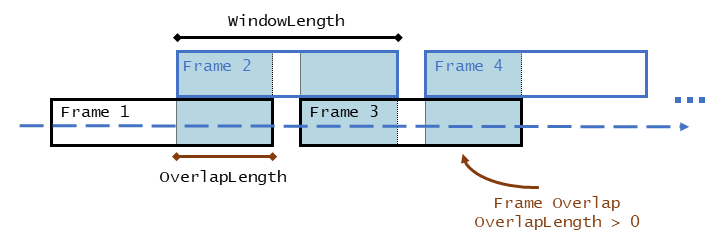
\includegraphics[width=1.1\linewidth]{mfcc_audioframes}
\caption{Audio Feature Extraction using sub-band audio frames}
\label{fig:mfcc_extraction}
\end{figure}

\subsection{\textbf{Pitch}}
Pitch estimates fundamental frequency of audio signal (See figure: \ref{fig:pitch_plot}). The pitch values are also estimated for an audio at sub-band levels for frames of length 30ms. For an audio sampled at 8K\si{\hertz} rate, this imply 240 samples per frame. To reduce the effect of windowing, an overlap of 60 samples in adjacent frames is considered (See figure:\ref{fig:mfcc_extraction}\cite{mathworks:mfcc}).

\begin{figure}
\centering
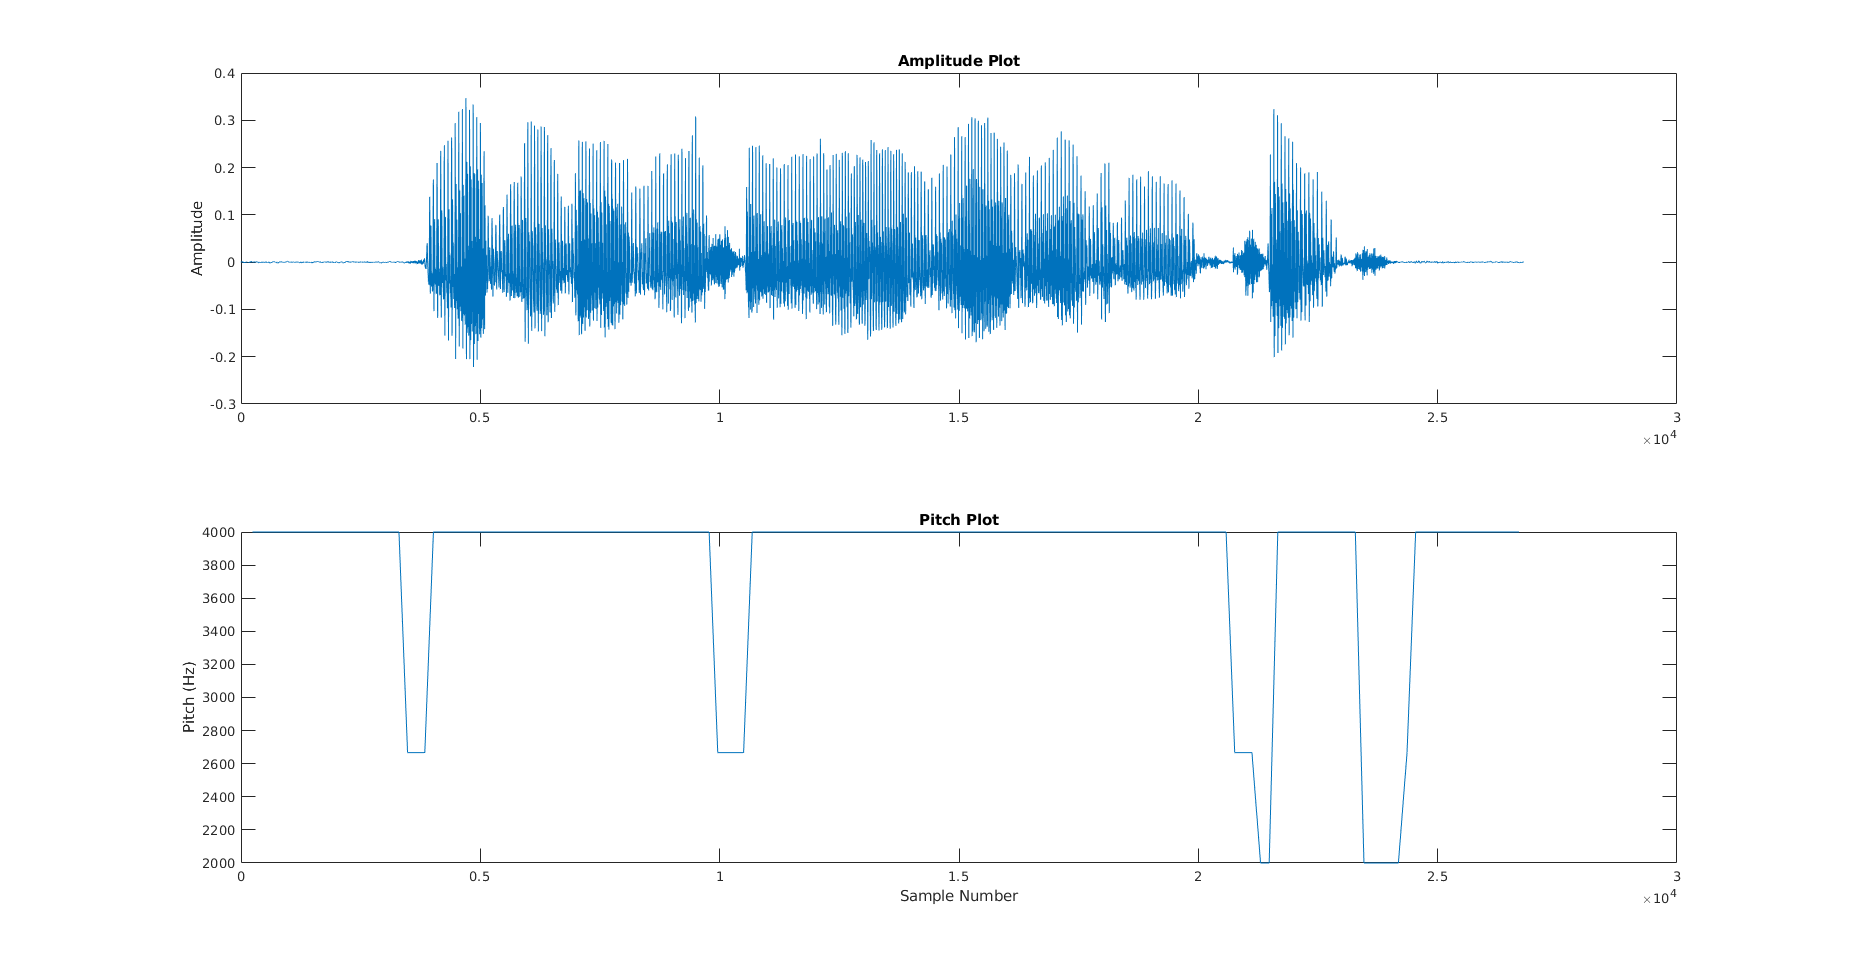
\includegraphics[width=1.2\linewidth]{pitch_plot}
\caption{Pitch plot for an audio waveform}
\label{fig:pitch_plot}
\end{figure}

\subsection{\textbf{Cochleagram}}
This is a representation of a  time-domain audio waveform in a t-f domain but is different from the spectrogram (See figure:\ref{fig:coch}). It is computed using an array of band pass filters that each model the frequency selectivity and nerve response of a single hair cell. Keeping this in mind, a 64 channel Gammatone filter bank as an array of band pass filters is used to estimate cochleagram.
Cochleagram evaluation involves using ERB (Equivalent Rectangular Bandwidth) as a psychoacoustic measure for approximating the frequency-dependent bandwidth of the filters in human hearing. The bandwidth of the rectangular bandpass filter is chosen such that it has the same peak and passes the same amount of power for an input of white noise.
\begin{figure}
\centering
\begin{subfigure}{.4\textwidth}
  \centering
  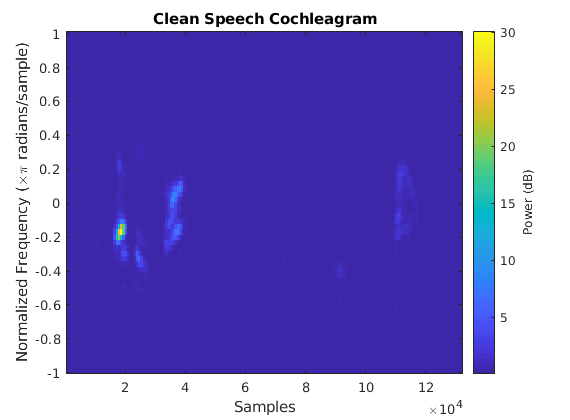
\includegraphics[width=1.1\linewidth]{clean_coch}
  \caption{Clean speech cochleagram}
  \label{fig:clean_coch}
\end{subfigure}%
\begin{subfigure}{.4\textwidth}
  \centering
  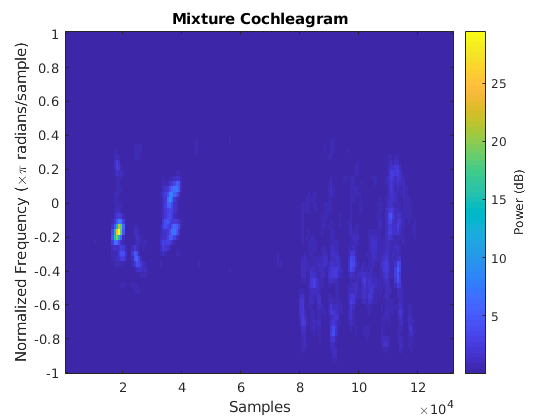
\includegraphics[width=1.1\linewidth]{mix_coch}
  \caption{Noisy mixture cochleagram}
  \label{fig:mix_coch}
\end{subfigure}
\begin{subfigure}{.4\textwidth}
  \centering
  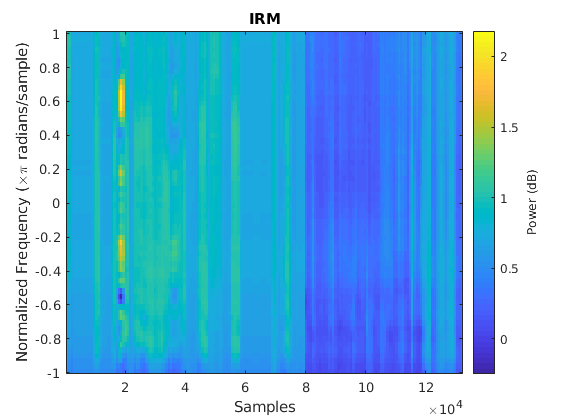
\includegraphics[width=1.1\linewidth]{irm_coch}
  \caption{IRM - by learning model}
  \label{fig:irm_coch}
\end{subfigure}
\begin{subfigure}{.4\textwidth}
  \centering
  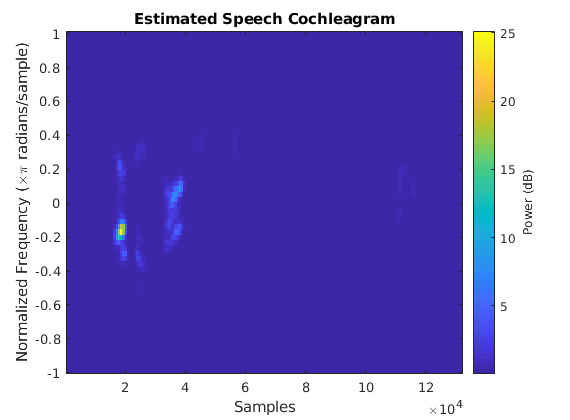
\includegraphics[width=1.1\linewidth]{estimated_coch}
  \caption{Estimated speech cochleagram}
  \label{fig:estimated_coch}
\end{subfigure}
\caption{Different stages of cochleagram during speech enhancement}
\label{fig:coch}
\end{figure}
%----------------------------------------------------------------------------------------

\section{Training Targets}
In supervised speech enhancement, defining a proper training target is important for learning and generalization. There are mainly two groups of training targets, i.e., masking-based targets and mapping-based targets. Masking-based targets describe the t-f relationships of clean speech to background interference, while mapping-based targets correspond to the spectral representations of clean speech. We focused on masking based training targets with a particular emphasis on usage of an \textbf{IRM} as a training target.\\
\subsection{IRM} 
IRM (Ideal Ratio Mask) is a soft mask \cite{ref:irm} which can be thresholded into a binary mask based on some local thresholding criterion. IRM is defined as:
\begin{equation}
IRM = \bigg( \frac{S(t,f)^2}{S(t,f)^2 + N(t,f)^2} \bigg)^\beta
\label{eq:irm}
\end{equation}
where $$S(t,f)^2$$ and $$N(t,f)^2$$ denote speech energy and noise energy within a T-F unit, respectively. The tunable parameter $$\beta$$ scales the mask, and is commonly chosen to 0.5. With the square root the IRM preserves the speech energy with each T-F unit, under the assumption that \textit{S(t,f)} and \textit{N(t,f)} are uncorrelated. Without the root the IRM in \ref{eq:irm} is similar to the classical Wiener filter, which is the optimal estimator of target speech in the power spectrum. An example of the IRM is shown in \ref{fig:irm_spect} and \ref{fig:irm_coch}.


